\documentclass[11pt,a4paper]{article}

\usepackage[T1]{fontenc}
\usepackage[utf8]{inputenc}
\usepackage[frenchb]{babel}

\usepackage{fancyhdr} % headers
\usepackage[usenames,dvipsnames]{color} % colors
\usepackage{graphicx} % images
\usepackage{listings} % source code
\usepackage{titling} % meta-infos
\usepackage{courier} % courier font
\usepackage{fullpage} % full page layout
\usepackage{titlesec} % title customization
\usepackage{parskip} % paragraphs spacing
%\usepackage{showframe} % layout debug

\topmargin=-10mm
\headsep=5mm
\headheight=10mm

\linespread{1.0}

\setlength\parindent{0pt}
\setlength{\unitlength}{1cm}
\setlength{\droptitle}{-1.6cm}

\pagestyle{fancy}
\fancyhf{}
\cfoot{\thepage}

\renewcommand{\thesection}{Problème \arabic{section} :}
\renewcommand{\thesubsection}{\arabic{section}.\arabic{subsection}}

\newcommand{\shellcmd}[1]{\texttt{\footnotesize\# #1}}

\def \doctitle { TIB-1-B \\ Labo 1: Wireshark }
\author{Bastien Clément \and Christophe Peretti}

\rhead{\theauthor \\ \today}
\lhead{\doctitle }
\title{\doctitle }

\begin{document}

\maketitle

\section{Wireshark et diagrammes}

L'objectif de ce premier exercice est d'apprendre à effectuer des captures simples avec le logiciel Wireshark, utiliser des filtres d'affichage puis documenter nos résultats à l'aide de diagrammes en flèche.

\subsection{Diagramme en flèche}

\begin{picture}(15,6.5)
\put(1.05,5.95){Ubuntu-11}
\put(0.8,5.45){10.192.72.127}
\put(7.1,5.95){Gmail}
\put(6.5,5.45){173.194.40.86}
\put(0.3,4.45){7.3165s}
\put(8.2,4.45){Client Hello}
\put(0.3,3.65){7.3240s}
\put(8.2,3.65){Server Hello}
\put(0.3,2.85){7.3252s}
\put(8.2,2.85){Certificate}
\put(0.3,2.05){7.3286s}
\put(8.2,2.05){Server Key, Server Hello done}
\put(0.3,1.25){7.3286s}
\put(8.2,1.25){Client Key, Change Cipher, Encrypted}
\put(0.3,0.45){7.3363s}
\put(8.2,0.45){Encrypted, Change Cipher, Encrypted}
\put(0,0){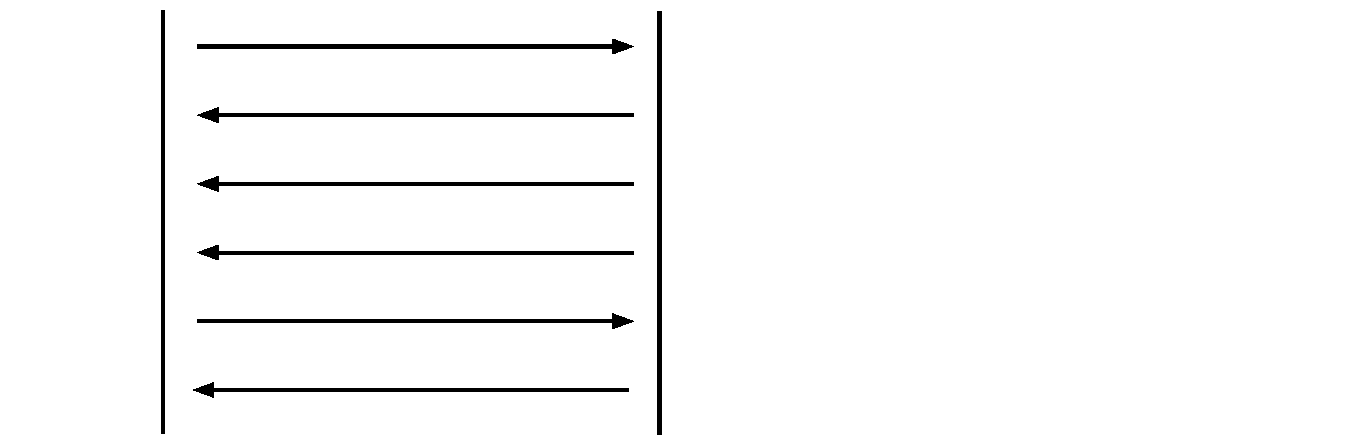
\includegraphics[width=\textwidth]{img_diagram2} }
\end{picture}

\section{Image cachée}

Ce second exercice a pour but d'apprendre à utiliser Wireshark pour analyser le trafic réseau généré par une requête HTTP et de trouver une image cachée parmi les données échangées.

Le protocole HTTP étant un protocole en mode texte (par opposition au mode binaire), il est relativement facile de lire les informations transmises en lisant directement la représentation ASCII des échanges entre le client et le serveur, facilement accessible par le menu contextuel de Wireshark.

\subsection{Requête HTTP}

La première étape est de localiser parmi les données collectée celles qui correspondent à la requête de la page contenant les indices menant à l'image cachée:

\texttt{GET http://iict-space.heig-vd.ch/jer/wschallenge/}

\subsection{Réponse HTTP}

La réponse du serveur est un relativement long document HTML dans lequel nous pouvons trouver le bloc de commentaires suivant:

\begin{verbatim}
	<!-- Felicitations ! Vous avez trouvée l'indice.    --><br />
	<!-- L'image se trouve sur                          --><br />
	<!-- http://iict-space.heig-vd.ch/jer/?p=29         --><br />
\end{verbatim}

Cette page contient en effet l'image cachée qu'il fallait trouver.

\subsection{Image}

\begin{center}

\includegraphics[width=3cm]{img_cachee}
\end{center}

\section{Analyse forensique}

Cet exercice à pour but d'apprendre à utiliser les fonctions avancées (conversations, flux) de Wireshark afin de répondre aux questions portant sur le contenu d'un email transmis sur le réseau à l'aide du protocole SMTP.

\subsection{Adresse d'Anne}

On peut observer qu'il y a deux messages différents dans les données interceptées. Le premier semble être destiné à un collègue d'Anne et le prévient qu'elle ne sera pas disponible pour un rendez-vous. Même si ce n'est pas le message qui nous intéresse, nous pouvons déjà en extraire l'adresse de Anne disponible dans les entêtes du message.

\texttt{From: \textbf{sneakyg33k@aol.com}}

\subsection{Adresse de l'amant secret}

Le second message est en revanche celui qui nous intéresse puisqu'il est destiné à l'amant secret et contient donc son adresse en tant que destinataire, toujours dans les entêtes du message.

\texttt{To: \textbf{mistersecretx@aol.com}}

\subsection{Objets demandés}

Un peut plus bas dans les données enregistrées, on peut voir qu'Anne demande à son amant d'apporter avec lui un \textbf{faux passeport} et un \textbf{costume de bain}.

\newpage

{\em Nous nous permettons de dépasser la limite de 2 pages afin de pouvoir inclure les résultats des exercices facultatifs.}

\section{Exercices avancés}

Ce dernier problème a pour but d'introduire des protocoles dont les données ne transitent pas directement en clair mais encodées. L'objectif est, encore une fois, d'extraire des informations à partir du trafic réseau enregistré. Cette fois-ci, le trafic n'est pas obtenu depuis notre propre activité mais récupéré d'une sessions enregistrée dans un fichier \texttt{.pcap}.

\subsection{Mot de passe}

Dans cet exercice, le client e-mail de Anne a choisi d'utiliser la méthode \texttt{AUTH LOGIN} pour s'authentifier avec le serveur. Conformément au protocole et aux indications du laboratoire, le nom d'utilisateur (son adresse e-mail) et le mot de passe sont transmis séquentiellement et sont encodés selon le format Base64.

Ce mot de passe peut être décodé avec la commande:

\shellcmd{echo "NTU4cjAwbHoK" | base64 -d}

Nous obtenons ainsi le mot de passe \textbf{558r00lz}.

\subsection{Ville du rendez-vous}

Dans le message envoyé à l'amant secret, nous pouvons observer une grande quantité de données encodées en Base64 à la fin du message transmis. Un regard plus attentif aux en-têtes permet de découvrir le type et le nom du document: \texttt{icantremember.docx}.

Le laboratoire suggère d'utiliser l'outil \texttt{munpack} pour extraire ce fichier. Cependant, n'ayant pas lu la donnée jusqu'au bout, nous avons extrait les données à la main dans un fichier \texttt{fichier.b64} puis décodé son contenu via la commande:

\shellcmd{cat fichier.b64 | base64 -d > fichier.docx}

Ce fichier contient une carte de la ville \textbf{Playa del Carmen}, au Mexique.

\end{document}